\chapter{Results and Discussion}
This chapter presents the findings of this work as well as the work that has been done and then discusses them in a wider context.

\section{Metadata structure}


Is this a sensible result representing reality and fulfilling demands in respect to working SHM and FAIR principles?

Thoughts on data structure flow.

A common ground has been found for the upload so that alterations to further processing parts of the cycle don't necessitate a full reupload of the original data. This common ground asserts that original is uploaded once with the downside that the DAQ configuration may not be fully interpretable at this stage due not being self describing metadata.

The following step of configuration solves this problem then by collecting and merging available metadata into a common scheme. This step works upon the DAQ metadata that is already uploaded to the skystash and then fuses it with other metadata sources that are locally available to generate a holistically valid metadataset. Notable is that this step will certainly be part of rather constant modification due to SHM configurations that are also provided within this step. Also the metadata schema is far from complete and will be in need of constant expansion to compensate the complex dimensions of flight test data as well as relevant test configuration data that also may be taken into consideration within this step \ref{fig:digecat_data_sources}. Since this step is far less computationally intensive than the parsing process this is considered as an acceptable tradeoff within this process.

This work's approach tries to implement the FAIR principles by using configuration files for the check algorithms that enable systemic control and extendability as well as by using a single source of truth, cleanly encapsulating every single step of the SHM process. However at the current point the metadata scheme is not clearly defined and work for a later point. Possible implementations may include the SOIL-scheme or other schemes that are possibly already suited for describing data quality and correlations. By also including the processing metadata configuration within the metadata, a reusability and traceability of the report logic is guaranteed.

An interactive frontend for the data report enables Accessibility of the SHM. Enabling a data quality overview for an entire flight dataset at a glance. Searchable metadata tags enable a dynamic search within the MongoDB Database.



\section{Check testing 1,2,3 (test with real data)}




Since the IMC DAQ System resamples the 20Hz Sensors to a straight timeframe data gets lost in the process. This makes potentially noisy sensors output the same value twice in a row since the DAQ hasn't yet received the new sensor data and outputs the same value multiple times in a row. Even sensors with a high noise ratio such as the fine part of a gps latitude signal outputs the same value twice in a row which is highly unlikely to happen on a statistical basis. Since this occurs quite often the question arises if the actual sampling may be lower than the actual data.


\subsection{Sensitivity Tuning}
%pasted from ch4
The validation loop is driven by previously known error types (See OneNote Sensor Errors)

It shows that while conservatively chosen ranges do not indicate many occurences, tighter limits enable more detailed monitoring.




Show plots of
\paragraph{Check with faulty data (Plots and comparisons)}
see onenote sensor errors

AE-errors
F89: FUS_050303

-stft from onenote. show progression from spectrogram to averaged amplitude over time


20210923_AVIA2ter Flug_(1): FUS_050303_pY, FUS_050209_pZ (offset), DFUS_230306

\begin{figure}
    \centering
    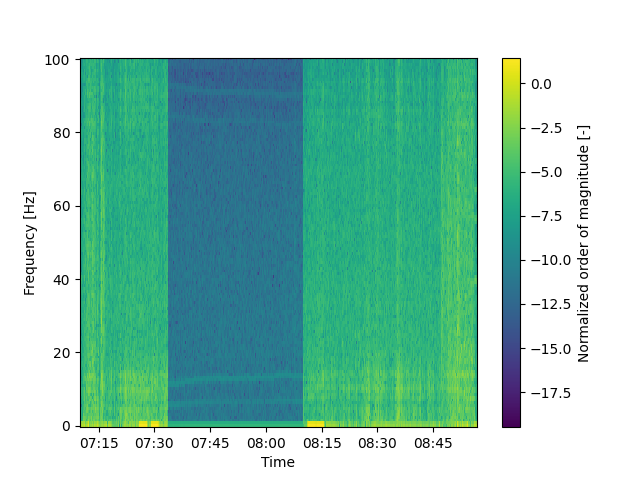
\includegraphics[width=.7\textwidth]{03_figures/python_functions/images/FUS_050303_spectro.png}
    \label{fig:res_050303_spectrogram}
    \caption{Capturing Errors}
\end{figure}



\begin{figure}
    \centering
    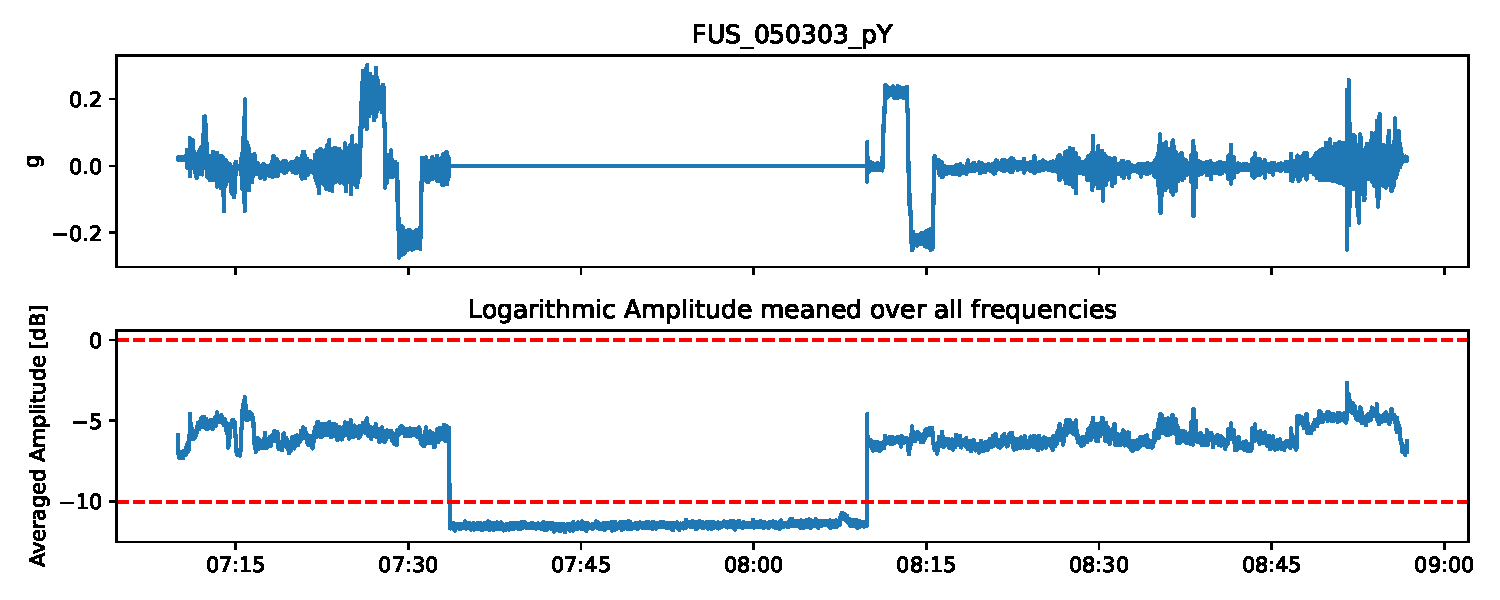
\includegraphics[width=.7\textwidth]{03_figures/python_functions/images/FUS_050303}
    \label{fig:res_050303}
    \caption{Capturing Errors}
\end{figure}

\begin{figure}
    \centering
    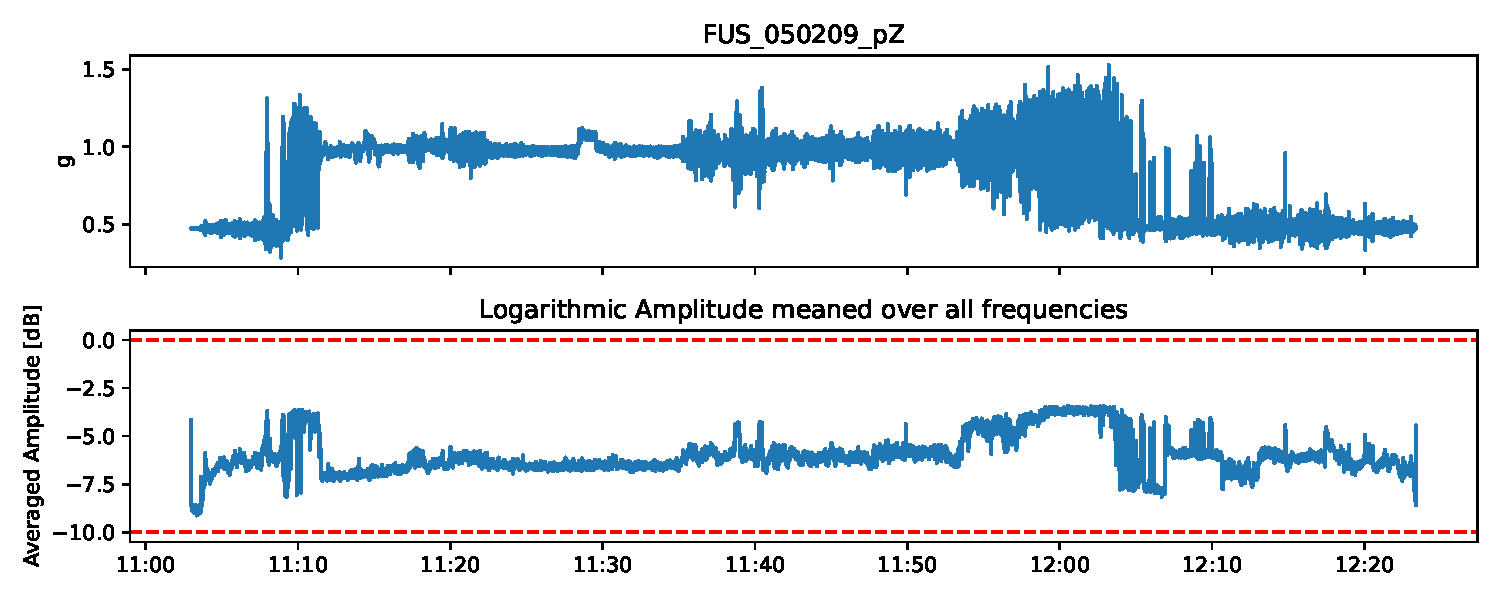
\includegraphics[width=.7\textwidth]{03_figures/python_functions/images/FUS_050209}
    \label{fig:res_050209}
    \caption{Capturing Errors}
\end{figure}






\subsection{Comparison with previously developed FMEAs}
PTF,Kalman,PCA

not nearly as good enough. However, focus of this work is to start off error detection within a FAIR context to generate interfaces for the skystash.

What could be reached with other FMEAs? Correlation Applications as well as Neural Networks.


\subsection{Rate check quality with parameters}
The data quality parameter fine tuning will still have to go a long way to fulfill all necessary and required conditions.

To summarize, the algorithms employed generally work by inspecting limits of parameter Series. These limits can also be set for modified parameter series that have e.g. been differentiated or fourier transformed. The interfaces have been created to allow for further implementation and optimization of parameters. The limits are defined within the configuration file (currently in excel format) and the Series transformation may also be customly defined.

As for general formats it has been found to be difficult to generalize for all parameter formats since many employ strictly discrete values. For error detection using single sensors only, it is possible to divide into the following categories: Value is out of bounds, the movement of the value is to high or the movement of the value is too low.

In level 3, fault tolerant sensors methods are employed that use hardware as well as analytical redundancy. \cite[p.355-365]{isermann_fault-diagnosis_2006}





\section{Implementation ecosystem}

How well is the implementation in the ecosystem? Modularity of components and extensibility with new functions.


-Embedding within the stash ecosystem. Clean Interfaces?



\subsection{Toolchain FTI-tool}
The following toolchain emerges for use of fti microservices.

Modular design allows encapsulation of algorithms as well as quick reaction towards faults and independence of fault modes.
I.e. wrong config does not require the data to be reuploaded.


\begin{figure}
    \centering
    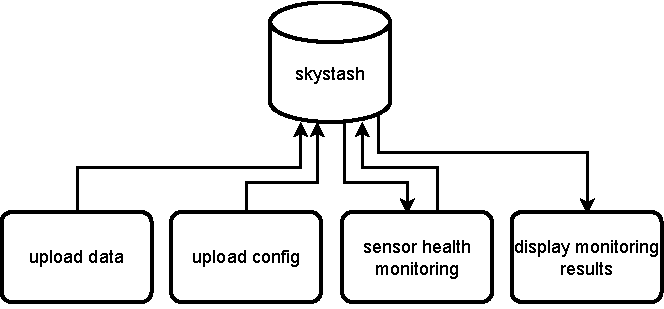
\includegraphics[width=.7\textwidth]{03_figures/FTI_microservices}
    \label{fig:fti-micro}
    \caption{The emerging FTI-Toolchain}
\end{figure}


\section{Discussion/Potential}

-lvl2:Of course, this topic could be examined within a depth that may exceed this work such as estimating white noise using discrete fourier Transform Subspace Decompositions \cite{hendriks_noise_2008} or statistical methods such as covariance operators.

The goal of this work however, is preservation of scalability, minimal user and configuration inputs.

Implementation list:tryouts
-lvl3 rigid body simulation for flight dynamics
-lvl3 implementation of multiple COS and their respective conversions
-lvl3 residual interpretation (better than highpass filtering and checking for std)

-Real time implementation
-Pseudo transfer functions (Generate a real time correlation matrix (MArkov parameters) and generate residuals based on that)
-PCA
-better parameter fusion algorithms (voting, or others see GNSS-RAIM)
        -aaim,
        -external factors integrity monitoring
- GANomaly approach (neural network) since an aircraft dataset is similar to images in that it is a multidimensional dataset

-more and better evaluation of the report display to satisfy innovation turbine requirements.


builds foundation for iot platforms that automatically can evaluate sensors, infrastructures and FMEAs. Since especially research data is highly customized this can be a possible way to deal with complex transformation functions as well as complex sensor/parameter interrelations.

\section{Conclusion}

These results show a promising prototype for a Sensor Health Monitoring Infrastructure. It establishes Interfaces and then
